\documentclass[a4paper]{article}
\usepackage[T1]{fontenc}
\usepackage[polish]{babel}
\usepackage[utf8]{inputenc}
\usepackage{lmodern}
\selectlanguage{polish}

\usepackage[margin=1 in, includefoot]{geometry}
\pagenumbering{arabic}
\setcounter{page}{2}
\usepackage{graphicx}
\usepackage{epsfig}
\usepackage{float}
\usepackage{multirow}
\usepackage[space]{grffile}
\usepackage{xcolor, listings}
\usepackage{mathtools}
\lstset{
basicstyle=\footnotesize\ttfamily,
numbers=left,
numberstyle=\tiny,
numbersep=5pt,
tabsize=2,
extendedchars=true,
breaklines=true,
commentstyle=\color{green},
keywordstyle=\color{blue},
identifierstyle=\color{black},
showspaces=false,
showstringspaces=false,
}
\lstdefinestyle{sharpc}{language=[Sharp]C, frame=lr, rulecolor=\color{blue!80!black}}
%nowa strona przed kazdym section
\let\oldsection\section
\renewcommand\section{\clearpage\oldsection}
\newcommand\tab[1][1cm]{\hspace*{#1}}

\renewcommand{\labelenumii}{\theenumii}
\renewcommand{\theenumii}{\theenumi.\arabic{enumii}.}

\begin{document}
\begin{titlepage}
\begin{center}
\huge{\textsc{Politechnika Wrocławska\\Wydział Elektroniki}}
\line(1,0){400}\\
[1 cm]
\textsc{\Huge {Zarządzanie w Systemach i Sieciach Komputerowych}}\\
[0.5 cm]
\textsc{\Large {Optymalizacja listy zakupów pod względem ceny}}\\
\end{center}
\vfill
\vfill
\hspace{0.5 cm}
\begin{minipage}[t]{.4\textwidth}%
\flushleft
\textsc{\Large{Autorzy :}}\\
\Large{Rafał Gubała }\\
\Large{Jakub Małyjasiak}
\end{minipage}%
\begin{minipage}[t]{.5\textwidth}%
\flushright
\textsc{\Large{Prowadzący :}}\\
\Large{dr inż. Robert Wójcik}\\
\end{minipage}%
\vfill
\begin{center}
\normalsize{Wrocław 2017}
\end{center}
\end{titlepage}

\tableofcontents 
\listoffigures

\section{Wstęp}
\subsection{Cel projektu}
\large
Celem projektu było opracowanie i stworzenie aplikacji na platformę Windows implementującą algorytmy optymalizujące listy zakupowe pod względem ceny produktów z różnych sklepów.
\subsection{Zakres projektu}
\large
Założenie projektowe obejmowały stworzenie aplikacji okienkowej posiadającej następujące funkcjonalności:
\begin{itemize}
\item Dodawanie, edycja oraz usuwanie sklepów
\item Dodawanie, edycja oraz usuwanie produktów
\item Tworzenie list zakupowych z wybranymi produktami
\item Optymalizacja list zakupowych algorytmami \textbf{Shop-Enum} oraz \textbf{Product-Enum}
\item Mierzenie czasu wykonywania się poszczególnych algorytmów
\item Zapisywanie i wczytywanie wprowadzonych danych
\end{itemize}
\section{Sformułowanie problemu}
\subsection{Podstawowe założenia}
\large
Rozwiązywany problem dotyczy zakupów internetowych i zminimalizowania kosztów poniesionych przy zakupie wybranych produktów w wybranych sklepach. Pojedyncza osoba szuka określonego zestawu produktów $N = \{1,...,n\}$ w $m$ sklepach. Każdy sklep posiada swój koszt wysyłki $d_i$ oraz każdy podzbiór produktów $N_i$ może być skojarzony z wieloma sklepami. Oprócz tego, każdy produkt należący do wybranego podzbioru $N_i$ posiada swoją cenę $c_{ji}$, gdzie $j \in N_i$ Rozwiązaniem problemu jest znalezienie takiego zestawu produktów z co najmniej jednego sklepu, aby sumaryczna wartość zakupów była jak najmniejsza.
\subsection{Opis wariantów problemu}
\subsubsection{Problem decyzyjny}
W przypadku obu algorytmów problem decyzyjny sprowadza się do pytania, czy istnieje podzbiór produktów $N_i$ i odpowiadający mu zbiór sklepów $M_i$, dla którego sumaryczny koszt zakupu będzie równy $k$. Rozwiązanie owego problemu będzie polegało na przeszukaniu zbioru wszystkich sklepów w poszukiwaniu produktów w podzbioru $N_i$. Jeśli wszystkie produkty udało się znaleźć, to sumując ceny wszystkich przedmiotów z cenami wysyłki w odpowiednich sklepach możemy udzielić odpowiedzi na postawione pytanie.
\subsubsection{Problem optymalizacyjny}
Mając na uwadze sformułowany wcześniej problem decyzyjny możemy prosto sformułować odpowiadający mu problem optymalizacyjny. W tym przypadku brzmi on: \textit{Ile wynosi najniższy koszt zakupu przedmiotów ze zbioru $N_i$ w zadanym zbiorze sklepów.} Warto zauważyć, że problem w istocie nie jest trywialny. Ważną komplikacją jest fakt, że pod uwagę trzeba wziąć koszt wysyłki danego produktu, co sprawia, że proste przeszukanie sklepów w celu znalezienia najtańszych ofert dla danego produktu nie ma sensu. Czasami bardziej opłacalne może okazać się kupienie droższego produktu, jeśli pozwoli to uniknąć poniesienia kosztów wysyłki w innym sklepie. 
\subsection{Zastosowane algorytmy}
Posiłkując się materiałami zawartymi w [3] do rozwiązania problemu wykorzystaliśmy algorytmy \textit{SHOP-ENUM} oraz \textit{PRODUCT-ENUM}. Oba pozwalają znaleźć optymalne rozwiązanie, ale dzieje się to kosztem złożoności obliczeniowej.

Podstawowym założeniem algorytmu \textit{SHOP-ENUM} jest skupienie się na sklepach, zamiast na produktach. Zakładamy tutaj, że analizie poddamy każdy możliwy podzbiór sklepów, co pozwoli w trywialny sposób przeszukać kolekcję w celu znalezienia najtańszej oferty na dany produkt z punktu widzenia pojedynczej iteracji. Jest to możliwe dzięki temu, że koszt wysyłki nie gra tutaj roli. Ze względu na to, że analizie zostanie poddany każdy podzbiór sklepów, czyli każda możliwa kombinacja kosztów wysyłki, możemy w naiwny sposób szukać podzbioru produktów o najniższej cenie. Koszt wysyłki zwiększa ową cenę o odpowiednią wartość i w ten sposób otrzymujemy rezultat działania algorytmu.
\vspace{0.5 cm}
\lstset{style=sharpc}
\begin{lstlisting}
foreach permutation of stores
		foreach product in shoppingList
			cheapestProduct <- stores.findCheapest(product)
			resultList.add(cheapestProduct)
		
		if resultList.Cost < bestSolution.Cost then
			bestSolution <- resultList
\end{lstlisting}
\vspace{0.5 cm}

Algorytm \textit{PRODUCT-ENUM} to przeciwieństwo wspomnianego wcześniej algorytmu \textit{SHOP-ENUM}. Tutaj uwagę skupia się na produktach. Podstawą algorytmu jest założenie, że tym razem zamiast analizować każdy możliwy podzbiór sklepów, stworzymy każdą możliwą kombinację produktów. Pseudokod trafnie obrazuje ten zamysł:

\vspace{0.5 cm}
\lstset{style=sharpc}
\begin{lstlisting}
Permutate(shoppingList, stores, itemIndex) {
	if itemIndex < shoppingList.Count then
		foreach store in stores 
			product <-  store.findProduct(shoppingList[itemIndex])
			if product.Amount < shoppingList[itemIndex].Amount then continue
			shoppingList[itemIndex].setNewPrice(product.Price)
			shoppingList[itemIndex].setNewStore(product.Store)
		
			Permutate(shoppingList, stores, itemIndex + 1)
	else
		if shoppingList.Cost < bestSolution.Cost then
			bestSolution <- shoppingList
}
\end{lstlisting}
\vspace{0.5 cm}
Widać tutaj jasno, że naszym zamiarem będzie stworzenie każdej możliwej kombinacji produktów, jak już wcześniej wspomniano. W praktyce oznacza to wykorzystanie rekurencji, która pozwoli na każdej pozycji na liście zakupów przeanalizować wariant, w którym produkt bierzemy kolejno z każdego sklepu, w którym jest dostępny
\subsection{Analiza złożoności obliczeniowej algorytmów}
\subsubsection{Algorytm SHOP-ENUM}
Zauważmy, że skoro algorytm bazuje na utworzeniu wszystkich możliwych kombinacji analizowanych sklepów ze zbioru $\{1,...,m\}$, to wszystkich możliwych kombinacji będzie $2^m$. Następnie należy znaleźć najtańszą ofertę na dany produkt, co w przypadku przechowywania sklepów na liście można otrzymać w czasie $O(m)$, jeśli m to ilość przeszukiwanych produktów. Mamy zatem $2^mm$. Operację wyszukiwania należy powtórzyć dla każdego produktu na liście zakupów, której długość możemy oznaczyć jako $n$. Mamy zatem ostatecznie
\begin{equation}
O(nm2^m)
\end{equation}
Dużą poprawę można byłoby osiągnąć, gdyby oferty produktów były przechowywane w kopcu. Wtedy operacja znalezienie najtańszej oferty, zakładając, że będzie to kopiec minimalny względem ceny, udałoby się wykonać w stałym czasie, a złożoność spadłaby do:
\begin{equation}
O(n2^m)
\end{equation}
\subsubsection{Algorytm PRODUCT-ENUM}
Algorytm \textit{PRODUCT-ENUM}, jak już wcześniej stwierdzono, polega na przeanalizowaniu każdego możliwego zbioru produktów. Jeśli oznaczymy ilość produktów na liście jako $n$, czyli produkty stworzą podzbiór $S = \{S_1,...,S_n\}$, a ilość sklepów przez $m$, to zauważymy, że istnieje $m^n$ takich kombinacji. Daje to złożoność równą $O(m^n)$. Na tym etapie, w przeciwieństwie do algorytmu \textit{SHOP-ENUM}, nie mamy jeszcze żadnej informacji o cenie produktów. Jeśli, jak już ustaliliśmy, podzbiór składa się z $n$ elementów, to dodając ten etap do dotychczasowej złożoności otrzymujemy:
\begin{equation}
O(nm^n)
\end{equation}
\section{Projekt aplikacji}
\subsection{Wykorzystywane technologie i narzędzia projektowania}
Do stworzenie projektu zostały użyte następujące technologie i narzędzia:
\begin{itemize}
\item Język programowania: C\#
\item Środowisko programistyczne: Visual Studio 2015, Visual Studio 2017
\item XAML - język opisu interfejsu użytkownika
\item Inne: WPF, NewtonSoft: JSON.Net
\end{itemize}
\subsection{Struktura programu}
W projekcie został zastosowany wzorzec obiektowy. Aplikacja została napisana z rozdzieleniem interfejsu użytkownika oraz logiki samych algorytmów minimalizujących w postaci odrębnych modułów (projektów w solucji). Zabieg ten miał na celu wyodrębnić moduł algorytmiczny, aby można go było łatwo przenieść w przyszłości do innego projektu np. w postaci skompilowanej biblioteki.
\begin{flushleft}
Program zapisuje dane do pliku tekstowego w popularnym formacie JSON. Umożliwia to łatwy odczyt i parsowanie tekstu do obiektów w programie. Jest to symulacja bazy danych. Obsługa danych została zrealizowana jako wzorzec fabryki, każda encja posiada swoją fabrykę z metodami takimi jak: \textit{getAll}, \textit{getByID}, \textit{create}, \textit{update} oraz \textit{delete}.
\end{flushleft}
\subsection{Koncepcja działania algorytmów}
Oba algorytmy, jak już wcześniej wspomniano, zostaną umieszczone w osobnym module, co pozwoli lepiej odseparować logikę od widoku oraz wykorzystać skompilowany kod w innych projektach. Dla uproszczenia zostaną wprowadzone dodatkowe obiekty, które lepiej pasują do realizacji algorytmów. 
\subsubsection{Algorytm SHOP-ENUM}
W przypadku tegoż algorytmu konieczne jest znalezienie sposobu na szybkie i oszczędne generowanie kolejnych podzbiorów analizowanych sklepów. Rozwiążemy to tworząc osobną strukturę – tablicę zmiennych logicznych, lub liczb całkowitych takich, ze $x \in \{0, 1\}$ – która będzie stanowiła swego rodzaju maskę bitową. Załóżmy, że  mamy zbiór $\{a, b, c, d\}$ sklepów, a na danym etapie analizie mają podlegać jedynie sklepy \textit{a} oraz \textit{d}. Wtedy maska będzie miała postać $[1, 0, 0, 1]$. Stosują odpowiednie algorytmy możemy regularnie przesuwać maskę uzyskując wszystkie możliwe kombinacje. Następnie konieczne będzie wyszukanie najtańszej oferty sprzedaży danego produktu w dostępnych w danej iteracji sklepach. Do przechowywania danych wykorzystujemy nieposortowane listy – każdy sklep ma listę dostępnych w nim produktów, więc konieczne będzie przejrzenie kolejno wszystkich elementów listy i znalezienie tego, który zawiera najniższą cenę. Cena ta może zostać od razu dodana do końcowej sumy, co pozwoli uniknąć kolejnego iterowania po liście zakupów.
\subsubsection{Algorytm PRODUCT-ENUM}
Ze względu na konieczność wygenerowania każdej możliwej kombinacji produkt – sklep najprostszym wyjściem jest zastosowanie rekurencji. Implementacja będzie musiała umożliwiać "rozgałęzianie" na każdej pozycji listy zakupów dla wszystkich sklepów, w których dany produkt jest dostępny i jeśli zostanie osiągnięty ostatni poziom drzewa, obliczyć ceny i zwrócić najkorzystniejszą. Takie rozwiązanie będzie miało znaczną złożoność pamięciową, ponieważ wskutek rekurencji powstanie drzewo o $n$ – poziomach, a każdy węzeł będzie miał maksymalnie $m$ – rozgałęzień, gdzie $n$ - ilość produktów na liście, a $m$ - ilość sklepów. Daje to $m^n$ węzłów końcowych.
\subsection{Diagram klas}
\begin{figure}[H]
\centering
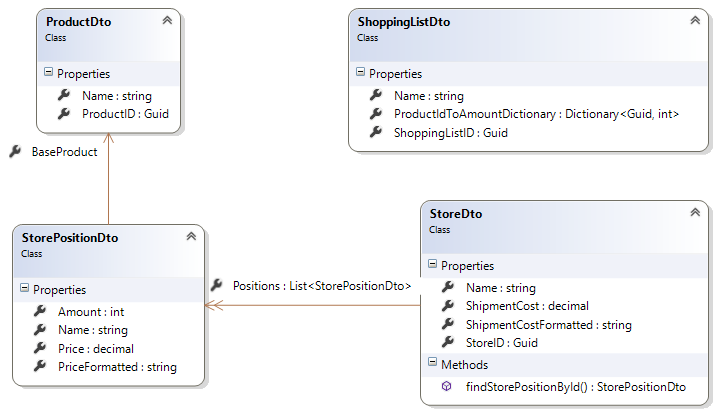
\includegraphics[width=\textwidth,keepaspectratio]{img/diagram-dto.png}
\caption{Diagram klas modeli używanych w module algorytmicznym}
\end{figure}
\begin{figure}[H]
\centering
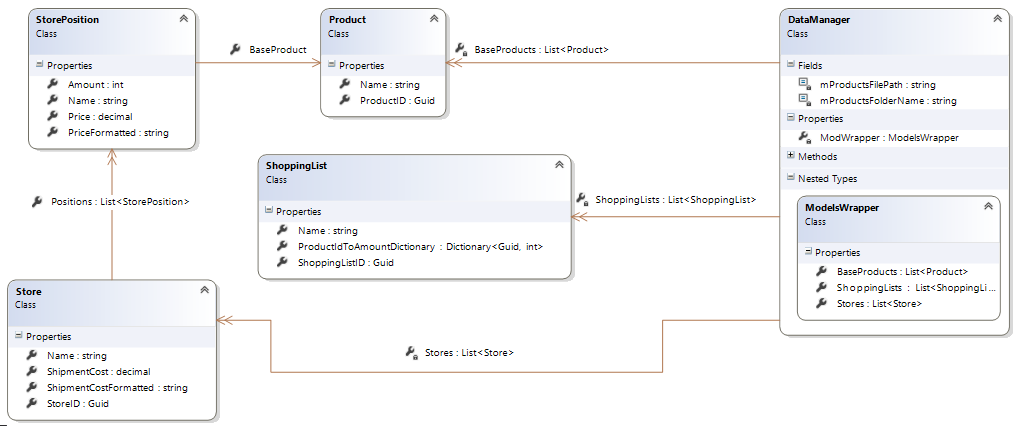
\includegraphics[width=\textwidth,keepaspectratio]{img/diagram-gui.png}
\caption{Diagram klas modeli używanych w interfejsie użytkownika}
\end{figure}
\subsection{Struktura danych wejściowych}
Struktura danych wejściowych algorytmu wygląda następująco:
\begin{itemize}
\item \textit{List<StoreDto> stores} - lista sklepów istniejących w bazie
\item \textit{Dictionary<Guid, int> productsIDToAmount} - słownik przyporządkowujący każdemu wybranemu produktowi (jego identyfikatorowi) z listy zakupowej ilość tego produktu zakupioną przez użytkownika
\item \textit{Algorithm algorithm} - typ wyliczeniowy informujący o tym jaki algorytm będzie zastosowany. Typ \textit{Algorithm} może przyjąć jedną wartość z dwóch do wyboru:
\newline \textit{\textbf{ShopEnum}} lub \textit{\textbf{ProductEnum}}
\end{itemize}
\subsection{Struktura wyników}
Algorytm zwraca obiekt typu \textbf{OptimizedShoppingList}, którego struktura i implementacja wygląda następująco:
\newline
\lstset{style=sharpc}
\begin{lstlisting}
public class OptimizedShoppingList
{
		public List<ShoppingListPosition> Products { get; set; }
    public TimeSpan TimeElapsed { get; set; }
    public decimal TotalPrice { get; set; }

    public OptimizedShoppingList()
    {
    	TotalPrice = decimal.MaxValue;
    }
}
\end{lstlisting}
\newpage
Klasa ta posiada 3 atrybuty:
\begin{itemize}
\item \textit{Products} - lista produktów wytypowanych przez algorytm. Każdy obiekt tej listy posiada informację z jakiego jest sklepu, swój identyfikator, cenę i ilość. Implementacja klasy obiektu z listy:
\newline
\begin{lstlisting}
public class ShoppingListPosition
{
		public StoreDto Store { get; set; }
    public Guid ProductId { get; set; }
    public decimal Price { get; set; }
    public int Amount { get; set; }
}  
\end{lstlisting}
\item \textit{TimeElapsed} - obiekt zawierający informacje o czasie wykonania się algorytmu
\item \textit{TotalPrice} - cena całościowa wytypowana przez algorytm
\end{itemize}
\section{Implementacja systemu}
\subsection{Wybrane klasy}
\subsubsection{ShoppingList}
\lstset{style=sharpc}
\begin{lstlisting}
public class ShoppingList
{
    public Guid ShoppingListID { get; set; }
    public string Name { get; set; }
		public Dictionary<Guid, int> ProductIdToAmountDictionary { get; set; }
}
\end{lstlisting}
\begin{flushleft}
Powyższa klasa reprezentuje listę zakupową. Posiada ona 3 pola: 
\begin{itemize}
\item \textit{ShoppingListID}: identyfikator zrealizowany za pomocą klasy \textbf{Guid} (zapewnia to bardzo dużą losowość)
\item \textit{Name}: nazwa list zakupowej
\item \textit{ProductIdToAmountDictionary}: słownik przyporządkowujący identyfikator produktu na liście do jego ilości
\end{itemize}
\end{flushleft}
\subsubsection{Store}
\lstset{style=sharpc}
\begin{lstlisting}
public class Store
{           
		public Guid StoreID { get; set; }
    public string Name { get; set; }
    public List<StorePosition> Positions { get; set; }
    public decimal ShipmentCost { get; set; }
    public string ShipmentCostFormatted
    {
    		get
        {
        		return this.ShipmentCost.ToString("C");
        }
     }
}
\end{lstlisting}
\begin{flushleft}
Powyższa klasa reprezentuje sklep. Posiada ona 5 pól: 
\begin{itemize}
\item \textit{StoreID}: identyfikator zrealizowany za pomocą klasy \textbf{Guid} 
\item \textit{Name}: nazwa sklepu
\item \textit{Positions}: lista przechowujące pozycje (produkty) sklepowe
\item \textit{ShipmentCost}: cena wysyłki
\item \textit{ShipmentCostFormatted}: sformatowana cena wysyłki, np. "15,00 zł"
\end{itemize}
\end{flushleft}
\subsubsection{Product}
\lstset{style=sharpc}
\begin{lstlisting}
public class Product
{     
	public Guid ProductID { get; set; }      
	public string Name { get; set; }        
}
\end{lstlisting}
\begin{flushleft}
Powyższa klasa reprezentuje produkt. Posiada ona 2 pola: 
\begin{itemize}
\item \textit{ProductID}: identyfikator zrealizowany za pomocą klasy \textbf{Guid} 
\item \textit{Name}: nazwa produktu
\end{itemize}
\end{flushleft}
\subsection{Realizacja algorytmów wyznaczania rozwiązań}
\subsubsection{Algorytm SHOP-ENUM}
Omówienie algorytmu zaczniemy od zaprezentowania kodu, który prezentuje się następująco.
\begin{lstlisting}
using System;
using System.Collections.Generic;
using System.Diagnostics;
using System.Threading;
using KnapsackOptimizer.Model;
using KnapsackOptimizer.Model.Dto;

namespace KnapsackOptimizer.ShopEnum.Logic
{
	public class ShopEnumAlgorithm
	{
		public OptimizedShoppingList Run(Dictionary<Guid, int> shoppingList, List<StoreDto> stores)
		{
			Stopwatch stopwatch = Stopwatch.StartNew();
			var bestShoppingList = new AlgorithmShoppingList(shoppingList);
			bestShoppingList.ComputeCost();
			var currentShoppingList = new AlgorithmShoppingList(shoppingList);

			var subsetMask = new int[stores.Count];

			while (GetNextPermutation(subsetMask) != 1)
			{
				for (var i = 0; i < stores.Count; i++)
				{
					if (subsetMask[i] == 0) continue;
					currentShoppingList.Products.ForEach(shopEnumPosition =>
					{
						stores[i].Positions.ForEach(position =>
						{
							if (position.BaseProduct.ProductID != shopEnumPosition.ProductId) return;
							if (position.Price >= shopEnumPosition.Price) return;
							if (position.Amount < shopEnumPosition.Amount) return;
							shopEnumPosition.Store = stores[i];
							shopEnumPosition.ProductId = position.BaseProduct.ProductID;
							shopEnumPosition.Price = position.Price;
						});
					});
				}
				currentShoppingList.ComputeCost();
				if (currentShoppingList.Cost < bestShoppingList.Cost)
				{
					var temp = currentShoppingList;
					currentShoppingList = bestShoppingList;
					bestShoppingList = temp;
				}
				currentShoppingList.Clear();
			}
			stopwatch.Stop();
			var stopwatchElapsed = stopwatch.Elapsed;
			stopwatch = null;
			return bestShoppingList.ToOptimizedShoppingList(stopwatchElapsed);
		}
		
		private int GetNextPermutation(int[] subsetMask)
		{
			int carry = 1;
			int index = 0;
			while (carry == 1 && index < subsetMask.Length)
			{
				subsetMask[index] += 1;
				carry = subsetMask[index] / 2;
				subsetMask[index] %= 2;
				index++;
			}

			return carry;
		}
	}
}
\end{lstlisting}
Jak widać, algorytm został podzielony na dwie części. Jedna, będąca szkieletem, odpowiada za obliczanie kolejnych kosztów i kompletowanie listy zakupów, a druga generuje kolejne kombinacje sklepów, które podlegają dalszej analizie, czyli wśród których szukamy produktów do skompletowania listy zakupów. 

Pierwsza, czyli szkielet, odpowiada są utworzenie listy zakupów, dla każdej wygenerowanej kombinacji sklepów, co zostało już wspomniane. Algorytm kończy działanie w momencie, kiedy wszystkie kombinacje zostały przejrzane. Zwraca wtedy najkorzystniejszą opcję, która jest przechowywana w zmiennej \textit{bestShoppingList}. Wewnątrz, każdy sklep, który jest analizowany w danej kombinacji, jest przeszukiwany w celu znalezienia ofert na dany przedmiot. Jeśli ów przedmiot znajduje się w sklepie, to jest sprawdzana jego cena i w przypadku, jeśli jest ona bardziej korzystna, niż do tej pory znaleziona, sklep zostaje powiązany z danym produktem. Po zakończeniu analizy danej kombinacji następuje obliczenie kosztu dla danej listy zakupów i jeśli udało się znaleźć wszystkie przedmioty oraz nowa cena jest niższa od dotychczasowego najlepszego rozwiązania, to aktualna lista i najlepsza zostają zamienione miejscami. Zamiana nie jest w tym przypadku niezbędna, ale pozwala uniknąć konieczności kolejnej alokacji pamięci. Wykorzystujemy dotychczas zaalokowaną strukturę.

\subsubsection{Algorytm PRODUCT-ENUM}
Opis realizacji modułu zaczniemy od zaprezentowania kodu. Wygląda on następująco.
\begin{lstlisting}
using System;
using System.Collections.Generic;
using System.Diagnostics;
using KnapsackOptimizer.Model;
using KnapsackOptimizer.Model.Dto;

namespace KnapsackOptimizer.ProductEnum.Logic
{
	public class ProductEnumAlgorithm
	{
		private AlgorithmShoppingList BestSolution;
		public OptimizedShoppingList Run(Dictionary<Guid, int> shoppingList, List<StoreDto> stores)
		{
			Stopwatch stopwatch = Stopwatch.StartNew();
			BestSolution = new AlgorithmShoppingList(shoppingList);    
			var shopEnumProducts = new AlgorithmShoppingList(shoppingList);
			Permutate(shopEnumProducts, stores, 0);
			stopwatch.Stop();
			return BestSolution.ToOptimizedShoppingList(stopwatch.Elapsed);
		}

		private void Permutate(AlgorithmShoppingList list, List<StoreDto> stores, int itemIndex)
		{
			if (itemIndex < list.Products.Count)
			{
				foreach (var store in stores)
				{
					var storePosition = store.findStorePositionById(list.Products[itemIndex].ProductId);
					if (storePosition.Amount < list.Products[itemIndex].Amount) continue;
					list.Products[itemIndex].Price = storePosition.Price;
					list.Products[itemIndex].Store = store;

					Permutate(list, stores, itemIndex + 1);
				}
			}
			else
			{
				list.ComputeCost();
				if (list.Cost >= BestSolution.Cost) return;
				BestSolution.Products = list.Products;
				BestSolution.Cost = list.Cost;
			}
		}
	}
}

\end{lstlisting}

Tym razem również algorytm został podzielony na dwie części, ale w przeciwieństwie do algorytm \textit{SHOP-ENUM}, główna funkcjonalność nie znajduje się w szkieletowej funkcji. Tym razem znacznie wygodniej było oprzeć się na rekurencji. W tym celu powstała wywoływana rekurencyjnie funkcja \textit{Permutate}. Rozwiązuje to problem wygenerowania wszystkich możliwych powiązań sklep-produkt. Innymi słowy, chcemy znaleźć wszystkie możliwe sposoby na zrealizowanie listy zakupów.

Funkcja \textit{Permutate} dostaje argumenty \textit{list, stores} oraz \textit{itemIndex}. \textit{List} to po prostu lista zakupów, na której zapisywane są powiązania produkt-sklep. \textit{Stores} to lista dostępnych sklepów, natomiast \textit{item index} odpowiada na pozycję na której funkcja ma dokonać rozgałęzienia. W praktyce polega to na tym, że dla każdej kolejnej pozycji na liście zakupów dokonujemy rozgałęzienia, z których każde odpowiada jednemu ze sklepów, w którym można dany produkt kupić. Funkcja kończy rozgałęzianie, jeśli \textit{item index} jest równy ilości przedmiotów na liście. Wtedy dla każdego rozgałęzienia, których jest $m^n$, obliczana jest cena, którą następnie porównujemy do najlepszej znalezionej.
\newpage
\subsection{Metoda odczytu danych wejściowych}
Dane wejściowe jak zostało to wspomniane wcześniej zapisywane są w formacie \textbf{JSON} do pliku tekstowego. Przykładowy fragment:
\begin{figure}[H]
\centering
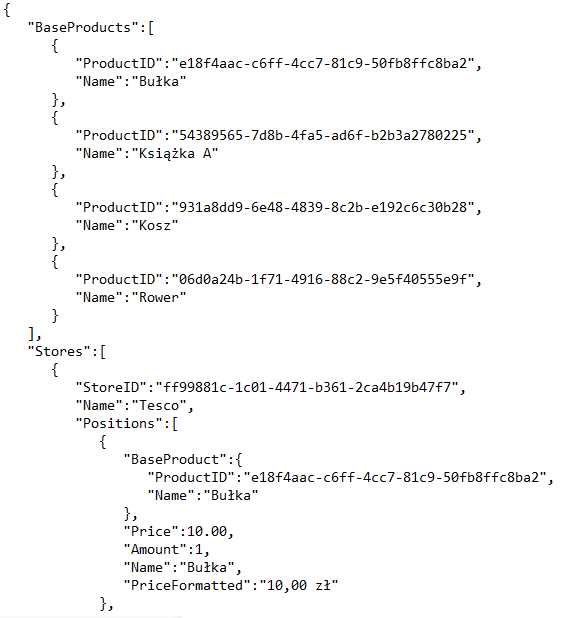
\includegraphics[width=\textwidth,keepaspectratio]{img/json.png}
\end{figure}
\newpage
Do odczytywania danych użyta została biblioteka \textbf{Json.NET - NewtonSoft}. W celu odczytania danych należało posłużyć się instrukcją:
\begin{lstlisting}
this.ModWrapper = JsonConvert.DeserializeObject<ModelsWrapper>(strJson)
\end{lstlisting} 
\begin{flushleft}
Obiekt \textit{ModWrapper} jest obiektem przechowującym dane przy zapisie lub odczycie. Przy odczycie biblioteka pobiera cały plik i deserializuje zapisanego tam JSON-a do obiektu. Struktura i implementacja obiektu \textit{ModWrapper} wygląda następująco:
\end{flushleft}
\begin{lstlisting}
private class ModelsWrapper
{
		public List<Product> BaseProducts { get; set; }
    public List<Store> Stores { get; set; }
    public List<ShoppingList> ShoppingLists { get; set; }
}
\end{lstlisting}
Klasa zawiera 3 atrybuty:
\begin{itemize}
\item \textit{BaseProducts} - lista produktów (sam wzorzec produktu)
\item \textit{Stores} - lista sklepów
\item \textit{ShoppingLists} - lista z obiektami reprezentującymi listy zakupowe
\end{itemize}
\subsection{Metoda prezentacji i zapisu wyników}
Dane prezentowane są zarówno w oknie głównym aplikacji jak i w pojedynczych mniejszych okienkach (popupach). Oto kilka przykładów:
\newline
\begin{figure}[H]
\centering
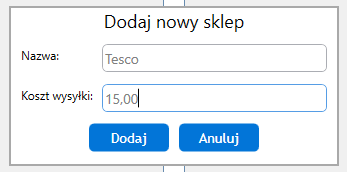
\includegraphics[width=\textwidth,keepaspectratio]{img/modal-nowy-sklep.png}
\caption{Dodawanie nowego sklepu}
\end{figure}
\begin{flushleft}
W tym oknie użytkownik może zdefiniować nowy sklep. Informacje, które należy podać to nazwa sklepu oraz koszt wysyłki produktów.
\end{flushleft}
\begin{figure}[H]
\centering
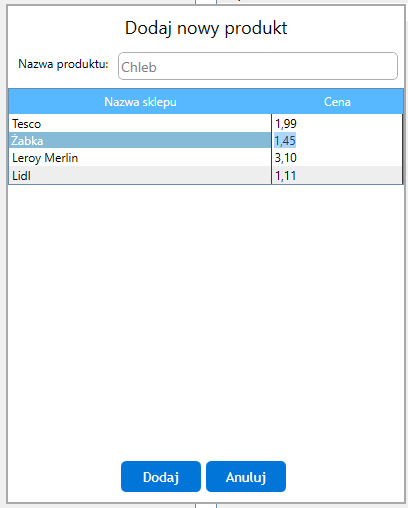
\includegraphics[width=\textwidth,keepaspectratio]{img/modal-nowy-produkt.png}
\caption{Dodawanie nowego produktu}
\end{figure}
\begin{flushleft}
W tym oknie użytkownik dodaje nowy produkt. Może wpisać jego nazwę oraz ile dany produkt kosztuje w każdym ze zdefiniowanych wcześniej sklepów.
\end{flushleft}
\begin{figure}[H]
\centering
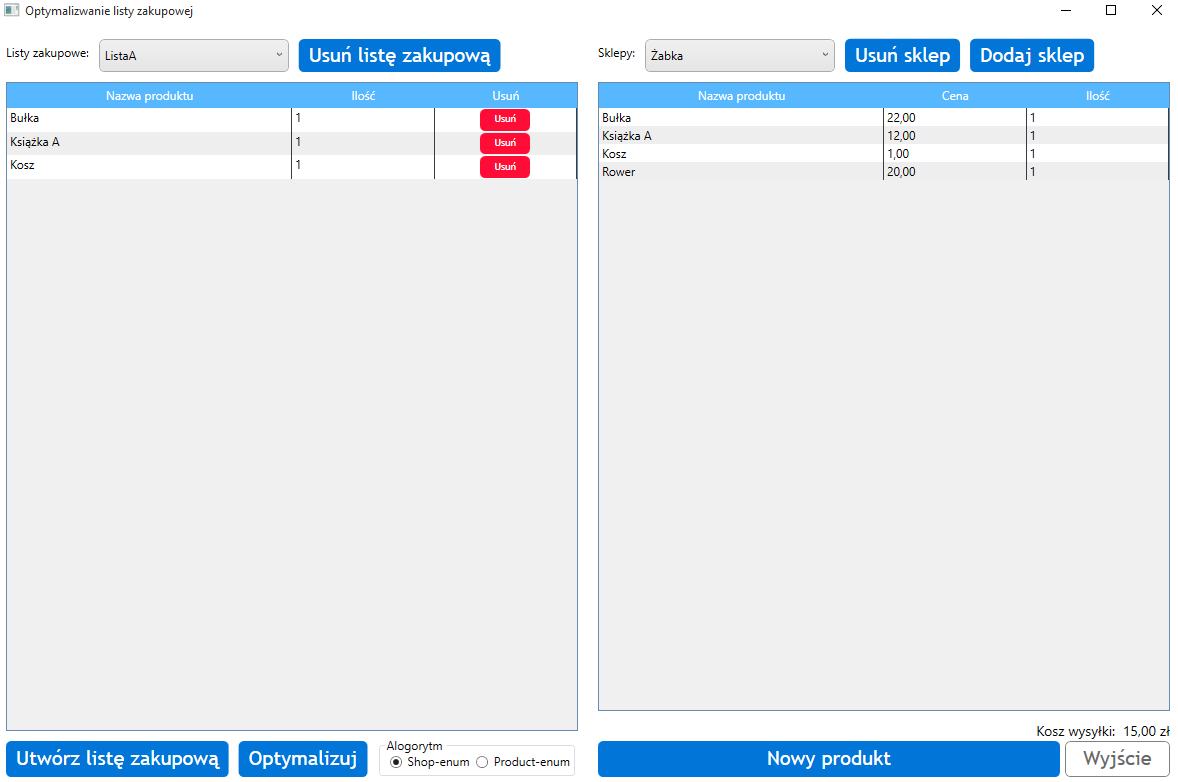
\includegraphics[width=\textwidth,keepaspectratio]{img/main.png}
\caption{Główne okno aplikacji z edycją list zakupowych oraz pozycji sklepowych}
\end{figure}
\begin{flushleft}
W głównym oknie aplikacji użytkownik może zarządzać listami zakupowymi, może je usuwać, zmieniać na nich produkty oraz usuwać produkty z listy. Listy zakupowe wybiera się z listy rozwijanej w lewym górnym rogu. W tym oknie można również zarządzać sklepami. Sklepy wybiera się z listy rozwijanej obok przycisku z napisem "Usuń sklep".
\end{flushleft}
\begin{figure}[H]
\centering
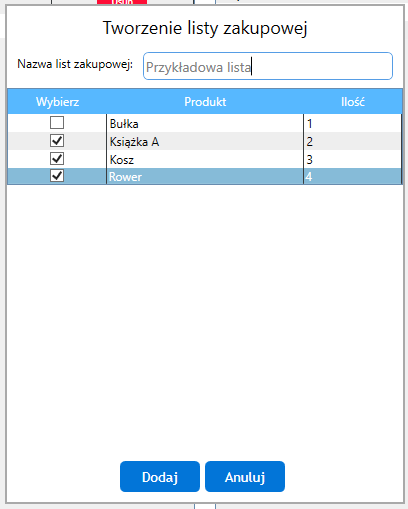
\includegraphics[width=\textwidth,keepaspectratio]{img/modal-nowa-lista.png}
\caption{Tworzenie listy zakupowej}
\end{figure}
\begin{flushleft}
W tym oknie użytkownik może wybrać, które istniejące produkty chce dodać do nowej listy zakupowej wraz z pożądaną ilością oraz może wpisać nazwę tej listy.
\end{flushleft}
\begin{figure}[H]
\centering
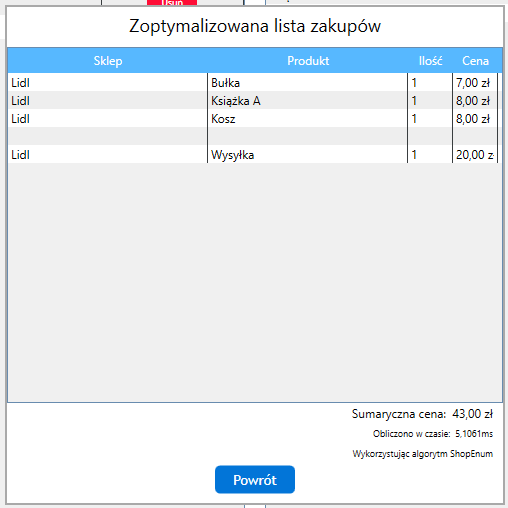
\includegraphics[width=\textwidth,keepaspectratio]{img/modal-optymalizacja.png}
\caption{Prezentacja wyniku algorytmu}
\end{figure}
\begin{flushleft}
Okno z wynikiem algorytmu prezentuje produkty, które zostały dodane do listy. Każdy produkt posiada informację z którego sklepu powinien być kupiony w celu optymalizacji kosztów. Okno to prezentuje również cenę sumaryczną za zakupy, czas poświęcony na optymalizację oraz informację jaki algorytm był użyty.
\end{flushleft}
\section{Testowanie poprawności i ocena rozwiązań}
\subsection{Testy jednostkowe}
W celu sprawdzenia poprawności działania algorytmu zostały sporządzone proste testy jednostkowe. Pozwoliło to upewnić się, że otrzymujemy oczekiwane wyniki, a algorytm zachowuje się zgodnie z przewidywaniami. Jako pierwszy zaprezentujemy test dla algorytmu \textit{SHOP-ENUM}.

\begin{lstlisting}
using System;
using System.Collections.Generic;
using KnapsackOptimizer.Model.Dto;
using Microsoft.VisualStudio.TestTools.UnitTesting;

namespace KnapsackOptimizer.ShopEnum.Logic.Tests
{
    [TestClass]
    public class ShopEnumAlgorithmTests
    {
        [TestMethod]
        public void RunTest()
        {
            //given
            var product1Id = Guid.NewGuid();
            var product1Amount = 1;
            var product1Name = "Product1Name";

            var product2Id = Guid.NewGuid();
            var product2Amount = 1;
            var product2Name = "Product1Name";

            var shop1Id = Guid.NewGuid();
            var shop1ShipmentCost = new decimal(10);

            var shop2Id = Guid.NewGuid();
            var shop2ShipmentCost = new decimal(20);

            var store1Dto = new StoreDto
            {
                ShipmentCost = shop1ShipmentCost,
                StoreID = shop1Id,
                Name = "Store1",
                Positions = new List<StorePositionDto>
                {
                    new StorePositionDto
                    {
                        Amount = 10,
                        Price = new decimal(35),
                        BaseProduct = new ProductDto
                        {
                            Name = product1Name,
                            ProductID = product1Id
                        }
                    },
                    new StorePositionDto
                    {
                        Amount = 10,
                        Price = new decimal(35),
                        BaseProduct = new ProductDto
                        {
                            Name = product2Name,
                            ProductID = product2Id
                        }
                    }
                }
            };

            var store2Dto = new StoreDto
            {
                ShipmentCost = shop2ShipmentCost,
                StoreID = shop2Id,
                Name = "Store2",
                Positions = new List<StorePositionDto>
                {
                    new StorePositionDto
                    {
                        Amount = 10,
                        Price = new decimal(5),
                        BaseProduct = new ProductDto
                        {
                            Name = product1Name,
                            ProductID = product1Id
                        }
                    },
                    new StorePositionDto
                    {
                        Amount = 10,
                        Price = new decimal(60),
                        BaseProduct = new ProductDto
                        {
                            Name = product2Name,
                            ProductID = product2Id
                        }
                    }
                }
            };
            var dictionary = new Dictionary<Guid, int>();
            dictionary.Add(product1Id, product1Amount);
            dictionary.Add(product2Id, product2Amount);

            var stores = new List<StoreDto> {store1Dto, store2Dto};

            //when
            var result = new ShopEnumAlgorithm().Run(dictionary, stores);

            //then
            Assert.AreEqual(result.TotalPrice, new decimal(70));
        }
    }
}
\end{lstlisting}
Poniżej natomiast znajduje się kod testu dla algorytmu \textit{PRODUCT-ENUM}. Nietrudno zauważyć, że poprawne wykonanie owych testów implikuje fakt, że wyniki zwracane przez oba algorytmy są nie tylko zgodne z oczekiwanymi, ale również ze sobą nawzajem.
\begin{lstlisting}
using System;
using System.Collections.Generic;
using KnapsackOptimizer.Model.Dto;
using KnapsackOptimizer.ProductEnum.Logic;
using Microsoft.VisualStudio.TestTools.UnitTesting;

namespace ShoppingOptimizerLogicTests.ProductEnum.Logic
{
    [TestClass]
    public class ProductEnumAlgorithmTests
    {
        [TestMethod]
        public void Run_WithValidData_ValidOutput()
        {
            //given
            var product1Id = Guid.NewGuid();
            var product1Amount = 1;
            var product1Name = "Product1Name";

            var product2Id = Guid.NewGuid();
            var product2Amount = 1;
            var product2Name = "Product1Name";

            var shop1Id = Guid.NewGuid();
            var shop1ShipmentCost = new decimal(10);

            var shop2Id = Guid.NewGuid();
            var shop2ShipmentCost = new decimal(20);

            var store1Dto = new StoreDto
            {
                ShipmentCost = shop1ShipmentCost,
                StoreID = shop1Id,
                Name = "Store1",
                Positions = new List<StorePositionDto>
                {
                    new StorePositionDto
                    {
                        Amount = 10,
                        Price = new decimal(25),
                        BaseProduct = new ProductDto
                        {
                            Name = product1Name,
                            ProductID = product1Id
                        }
                    },
                    new StorePositionDto
                    {
                        Amount = 10,
                        Price = new decimal(35),
                        BaseProduct = new ProductDto
                        {
                            Name = product2Name,
                            ProductID = product2Id
                        }
                    }
                }
            };

            var store2Dto = new StoreDto
            {
                ShipmentCost = shop2ShipmentCost,
                StoreID = shop2Id,
                Name = "Store2",
                Positions = new List<StorePositionDto>
                {
                    new StorePositionDto
                    {
                        Amount = 10,
                        Price = new decimal(5),
                        BaseProduct = new ProductDto
                        {
                            Name = product1Name,
                            ProductID = product1Id
                        }
                    },
                    new StorePositionDto
                    {
                        Amount = 10,
                        Price = new decimal(60),
                        BaseProduct = new ProductDto
                        {
                            Name = product2Name,
                            ProductID = product2Id
                        }
                    }
                }
            };


            var dictionary = new Dictionary<Guid, int>();
            dictionary.Add(product1Id, product1Amount);
            dictionary.Add(product2Id, product2Amount);

            var stores = new List<StoreDto> {store1Dto, store2Dto};

            //when
            var result = new ProductEnumAlgorithm().Run(dictionary, stores);

            //then
            Assert.AreEqual(result.TotalPrice, new decimal(70));
            Assert.AreEqual(result.Products.Count, 2);
            Assert.IsNotNull(result.Products[1].Store);
            Assert.AreNotEqual(result.Products[0].Price, Decimal.MaxValue);
        }
    }
}
\end{lstlisting}

\subsection{Weryfikacja poprawności działania algorytmów - przykłady}
Do udowodnienia poprawności algorytmów wykorzystamy następujący zbiór danych:

\begin{table}[H]
\renewcommand{\arraystretch}{1.3}
\centering
\caption{Przykładowe sklepy}
\begin{tabular}{|c|c|}
\hline
Sklepy & Cena wysyłki \\ \hline
Sa     & 10           \\ \hline
Sb     & 20           \\ \hline
\end{tabular}
\end{table}

\begin{table}[H]
\renewcommand{\arraystretch}{1.3}
\centering
\caption{Przykładowe produkty}
\begin{tabular}{|c|c|c|c|c|}
\hline
\multirow{3}{*}{Sklepy} & \multicolumn{4}{c|}{Produkty}                     \\ \cline{2-5} 
                        & \multicolumn{2}{c|}{p1} & \multicolumn{2}{c|}{p2} \\ \cline{2-5} 
                        & Ilość       & Cena      & Ilość       & Cena      \\ \hline
Sa                      & 10          & 35        & 10          & 35        \\ \hline
Sb                      & 10          & 5         & 10          & 60        \\ \hline
\end{tabular}
\end{table}

\begin{table}[H]
\renewcommand{\arraystretch}{1.3}
\centering
\caption{Lista zakupów}
\begin{tabular}{|c|c|}
\hline
Produkt & Ilość \\ \hline
p1      & 1     \\ \hline
p2      & 1     \\ \hline
\end{tabular}
\end{table}

Spodziewamy się zatem otrzymania w wyniku działania algorytmu następującej listy powiązań sklepów z produktami.

\begin{table}[H]
\renewcommand{\arraystretch}{1.3}
\centering
\caption{Rezultat działania algorytmu}
\begin{tabular}{|c|c|}
\hline
Produkt & Sklep \\ \hline
p1      & Sb    \\ \hline
p2      & Sa    \\ \hline
\end{tabular}
\end{table}

Ostateczny koszt zakupów powinien zatem wynosić 70, a składać będzie się na niego koszt produktu p1 w sklepie Sb (5), koszt produktu p2 w sklepie Sa (35), koszt wysyłki ze sklepu Sa (10) oraz koszt wysyłki ze sklepu Sb (20). Warto zauważyć, że taki dobór danych jest relatywnie prosty, ale pozwala wykryć błędy podczas dobierania przedmiotów.

\subsubsection{Algorytm SHOP-ENUM}
Przebieg algorytmu dla powyższej struktury będzie wyglądał następująco:
\begin{enumerate}
\item {$best \leftarrow empty list$, $subsetMask \leftarrow int[m]\{0\}$}
\item{ Przy inicjalizacji każdy produkt otrzymuje wstępną cenę równą maksymalnej wartości zmiennej Decimal tak, aby w dalszych krokach pierwsze znalezienie przedmiotu zaowocowało powiązaniem produktu z pierwszą znalezioną ofertą}
\item {Wygeneruj pierwszą kombinację w postaci maski, czyli $subsetMask \leftarrow \{0, 1\}$
\begin{enumerate}
\item {Teraz następuje iteracja po liście sklepów, i jeśli na odpowiednim indeksie w masce jest "1", to sklep zostaje wzięty pod uwagę. W tym przypadku pierwszy sklep zostaje poddany analizie, a drugi już nie. Przeszukując dostępne w nim produkty znajdujemy oba, których szukamy i dokonujemy powiązania, ponieważ cena jest lepsza}
\item{W tym momencie, dokonaniu dwóch powiązań, struktura danych je przechowująca ma postać.
$current \leftarrow \{(p1, Sa), (p2, Sa)\}$ i sumaryczny koszt równy 80.}
\item {Porównaj koszt aktualnej listy z najlepszą. Najlepsza nie została jeszcze zainicjalizowana, więc jest kosz jest równy maksymalnej wartości typu decimal. Warunek jest spełniony, więc listy są zamieniane miejscami, a nowa aktualna lista jest czyszczona.}
\end{enumerate}}
\item {Wygeneruj drugą kombinację w postaci maski, czyli $subsetMask \leftarrow \{1, 0\}$
\begin{enumerate}
\item {Tym razem tylko sklep Sb jest brany pod uwagę. Przeglądając go i porównując ceny do znajdujących się na aktualnej liście, która została wcześniej wyczyszczona (produkty mają cenę max decimal), wszystkie znalezione możemy powiązać}
\item{W tym momencie, dokonaniu dwóch powiązań, struktura danych je przechowująca ma postać.
$current \leftarrow \{(p1, Sb), (p2, Sb)\}$ i sumaryczny koszt równy 75.}
\item {Porównaj koszt aktualnej listy z najlepszą. Najlepsza lista po wykonaniu kroku 3.3 ma wartość 80, więc warunek jest spełniony. Listy zostają zamienione, a nowa aktualna jest czyszczona.}
\end{enumerate}}
\item {Wygeneruj trzecią kombinację w postaci maski, czyli $subsetMask \leftarrow \{1, 1\}$
\begin{enumerate}
\item {Tym razem oba sklepy są analizowane. Zaczynami od Sa, ponieważ ma niższy indeks. Przeglądając go i porównując ceny do znajdujących się na aktualnej liście, która została wcześniej wyczyszczona (produkty mają cenę max decimal), wszystkie znalezione możemy powiązać}
\item{W tym momencie, dokonaniu dwóch powiązań, struktura danych je przechowująca ma postać.
$current \leftarrow \{(p1, Sa), (p2, Sa)\}$.}
\item{Następnie przeglądamy oferty ze sklepu Sb. P1 kosztuje tutaj 5, podczas gdy wcześniej kosztował 35. Nie interesuje nas koszt wysyłki, więc bierzemy zawsze tańszy produkt. P2 jest droższy, niż w Sa, więc nie bierzemy go. Struktura przechowująca powiązania ma postać.
$current \leftarrow \{(p1, Sb), (p2, Sa)\}$ i sumaryczny koszt równy 70.}
\item {Porównaj koszt aktualnej listy z najlepszą. Najlepsza lista po wykonaniu kroku 4.3 ma wartość 75, więc warunek jest spełniony. Listy zostają zamienione, a nowa aktualna jest czyszczona.}
\end{enumerate}}
\item{ Kolejne wygenerowanie maski spowoduje przepełnienie, więc algorytm kończy działanie i zwraca aktualnie najlepszą listę. Jak widać ma ona taką samą cenę oraz powiązania, jak poszukiwana.}
\end{enumerate}

\subsubsection{Algorytm PRODUCT-ENUM}
\subsection{Analiza czasów wykonania algorytmów}
Czasy wykonania algorytmów zostały przeprowadzone dla relatywnie niewielkiej ilości zarówno sklepów, jak i produktów. Jest to spowodowane bardzo szybko rosnącym czasem wykonania. Oba algorytmy dają optymalne rozwiązanie, czego nie da się osiągnąć razem z wielomianowo rosnącym czasem. Konkretyzując, pomiary zostały przeprowadzone dla ilości sklepów $m \in \{8, 10, 12, 16\}$, a ilość \textit{n} produktów na liście była obliczana na podstawie ilości wszystkich dostępnych produktów. Założono, że ilość wszystkich produktów $p \in \{8, 10, 12\}$, a stosunek długości $n$ listy zakupów do wszystkich produktów będzie równy $d \in \{0.3, 0.7\}$. Przykładowo, jeśli liczba wszystkich produktów była równa $8$, to pomiary przeprowadzono dla $n=0.3 \cdot p=0.3 \cdot 8 = 2$ oraz $n=0.7 \cdot p=0.7 \cdot 8 = 6$. 

Pomiary zostały wykonane na maszynie pracującej pod systemem Windows 10 Pro. Wykorzystany sprzęt to procesor Intel core i7-6500U o taktowaniu 2,5GHz (3,1 GHz w trybie turbo), dwóch rdzeniach i 4MB pamięci podręcznej trzeciego poziomu oraz 8GB pamięci RAM DDR3L. Pozostałe specyfikacje nie grają kluczowych ról. Pomiary dla każdej konfiguracji parametrów zostały powtórzone 100 razy z małymi wyjątkami. Niektóre konfiguracje implikowały zbyt długi czas wykonania, przez co ilość powtórzeń była ograniczana. Zostanie do odnotowane w odpowiednich miejscach w dalszej części sprawozdania. Podczas wykonywania pomiarów jedynymi aktywnymi procesami, poza należącymi do testowanego programu, były procesy systemowe. Aplikacja nie była przystosowana do pracy wielowątkowej, przez co procesor był w stanie równomiernie, pod względem czasu, obciążyć każdy z rdzeni, dzięki czemu temperatura pozostała w rozsądnych granicach. Wersja wykonywalna programu, który podlegał testom, została skompilowana w trybie Release dla architektury 64-bitowej przy pomocy kompilatora wbudowanego w IDE Visual Studio 2017 Enterprise. Liczbowe wyniki pomiarów znajdują się w poniższej tabeli. Wykorzystano w niej wprowadzone wcześniej oznaczenia.

\begin{table}[H]
\centering
\caption{Tabela wszystkich pomiarów}
\renewcommand{\arraystretch}{1.3}
\begin{tabular}{|c|c|c|c|c|c|}
\hline
m {[}szt{]}         & p {[}szt{]}         & d   & n {[}szt{]} & shop-enum {[}ms{]} & product-enum {[}ms{]} \\ \hline
\multirow{6}{*}{8}  & \multirow{2}{*}{8}  & 0,3 & 2           & 0.025              & 0.030                 \\ \cline{3-6} 
                    &                     & 0,7 & 6           & 0.125              & 364.954               \\ \cline{2-6} 
                    & \multirow{2}{*}{10} & 0,3 & 3           & 0.106              & 0.356                 \\ \cline{3-6} 
                    &                     & 0,7 & 7           & 0.326              & 3406.234              \\ \cline{2-6} 
                    & \multirow{2}{*}{12} & 0,3 & 4           & 0.297              & 3.802                 \\ \cline{3-6} 
                    &                     & 0,7 & 8           & 0.985              & 31142.707             \\ \hline
\multirow{6}{*}{10} & \multirow{2}{*}{8}  & 0,3 & 2           & 9.362              & 0.046                 \\ \cline{3-6} 
                    &                     & 0,7 & 6           & 21.236             & 1392.188              \\ \cline{2-6} 
                    & \multirow{2}{*}{10} & 0,3 & 3           & 18.362             & 0.696                 \\ \cline{3-6} 
                    &                     & 0,7 & 7           & 41.236             & 16242.188             \\ \cline{2-6} 
                    & \multirow{2}{*}{12} & 0,3 & 4           & 36.663             & 9.281                 \\ \cline{3-6} 
                    &                     & 0,7 & 8           & 78.363             & 185625.000            \\ \hline
\multirow{6}{*}{12} & \multirow{2}{*}{8}  & 0,3 & 2           & 596.366            & 0.067                 \\ \cline{3-6} 
                    &                     & 0,7 & 6           & 1436.631           & 4157.050              \\ \cline{2-6} 
                    & \multirow{2}{*}{10} & 0,3 & 3           & 1298.378           & 1.203                 \\ \cline{3-6} 
                    &                     & 0,7 & 7           & 2859.120           & 58198.694             \\ \cline{2-6} 
                    & \multirow{2}{*}{12} & 0,3 & 4           & 2554.233           & 19.246                \\ \cline{3-6} 
                    &                     & 0,7 & 8           & 5632.245           & 798153.523            \\ \hline
\multirow{6}{*}{16} & \multirow{2}{*}{8}  & 0,3 & 2           & 41259.367          & 0.119                 \\ \cline{3-6} 
                    &                     & 0,7 & 6           & 116326.731         & 23357.030             \\ \cline{2-6} 
                    & \multirow{2}{*}{10} & 0,3 & 3           & 95682.511          & 2.851                 \\ \cline{3-6} 
                    &                     & 0,7 & 7           & 269861.282         & 435997.901            \\ \cline{2-6} 
                    & \multirow{2}{*}{12} & 0,3 & 4           & 223564.147         & 60.826                \\ \cline{3-6} 
                    &                     & 0,7 & 8           & 498623.214         & 7972533.043           \\ \hline
\end{tabular}
\end{table}

\begin{figure}[H]
\centering
\includegraphics[width=0.75\textwidth,keepaspectratio]{img/s8.eps}
\caption{Wykres czasu wykonania dla m=8}
\end{figure}

Zaprezentowany powyżej wykres jest oczywiście bardzo nieczytelny. Jest to spowodowane faktem, że algorytm \textit{PRODUCT-ENUM} jest bardzo czasochłonny, jeśli wzrasta długość listy zakupów. Jak widać, dla najniższej długości listy jest on bardzo zbliżony do pozostałych. Przybliżmy zatem pozostałe wartości.

\begin{figure}[H]
\centering
\includegraphics[width=0.75\textwidth,keepaspectratio]{img/s8zoom.eps}
\caption{Wykres czasu wykonania dla m=8 - przybliżenie}
\end{figure}

Bliższe spojrzenie na czasy wykonania pokazuje, że dla krótkich list zakupów algorytmy są bardzo zbliżone. Jest to jednak prawdą tylko, jeśli liczba sklepów jest niewielka, co jednoznacznie pokażemy na dalszych wykresach.

\begin{figure}[H]
\centering
\includegraphics[width=0.75\textwidth,keepaspectratio]{img/s10.eps}
\caption{Wykres czasu wykonania dla m=10}
\end{figure}

Powyższy wykres potwierdza olbrzymią różnicę na niekorzyść algorytmu \textit{PRODUCT-ENUM}, jeśli wzrasta ilość produktów na liście. Jako, że jest to w tym momencie pewne, pozwolimy sobie pominąć te pomiary na wykresach i ogarniczymy się do przypadków, w których porównanie jest możliwe i uzasadnione. Podobnie, jak poprzednio, skupmy się na porównaniu dla krótszej listy zakupów, gdyż powyższa ilustracja nie pozostawia wątpliwości w kwestii przypadku dłgiej listy.

\begin{figure}[H]
\centering
\includegraphics[width=0.75\textwidth,keepaspectratio]{img/s10zoom.eps}
\caption{Wykres czasu wykonania dla m=10 - przybliżenie}
\end{figure}

Po przybliżeniu i przyjrzeniu się zachowaniu algorytmów dla krótkich list zakupów można zauważyć, że algorytm \textit{PRODUCT-ENUM} jest znacznie bardziej efektywny, niż algorytm \textit{SHOP-ENUM}. W następnej przeprowadzonej analizie pozwolimy sobie pominąć diametralnie odstający od pozostałych wykres algorytmu \textit{PRODUCT-ENUM} dla wartości $d=0.7$.

\begin{figure}[H]
\centering
\includegraphics[width=0.75\textwidth,keepaspectratio]{img/s12zoom.eps}
\caption{Wykres czasu wykonania dla m=12}
\end{figure}

Zwiększenie ilości miast do 12 jeszcze bardziej wyeksponowało różnice wynikające z długości listy zakupów. Algorytm \textit{SHOP-ENUM} potrzebuje znacznie więcej czasu na wygenerowanie wszystkich możliwych kombinacji sklepów, których w tym przypadku jest $2^12$, czyli $4096$. W tym samym czasie, główny problem algorytmu \textit{PRODUCT-ENUM}, czyli generowanie wszystkich możliwych kombinacji sklep-produkt, daje nam $m^n$, czyli, dla najkrótszej listy, $12^2=144$ kombinacje. Nie ma wątpliwości, co do powodu dużych różnic w czasie wykonania.

\begin{figure}[H]
\centering
\includegraphics[width=0.75\textwidth,keepaspectratio]{img/s16zoom.eps}
\caption{Wykres czasu wykonania dla m=16}
\end{figure}

Jak widać na powyższym wykresie, kolejne zwiększenie ilości sklepów jeszcze bardziej zaogniło różnicę. Wszystko zostało już w tej kwestii powiedziane, więc zaprezentujmy jeszcze miejsce, w którym przecinają się wykresy obu algorytmów

\begin{figure}[H]
\centering
\includegraphics[width=0.75\textwidth,keepaspectratio]{img/s10extended.eps}
\caption{Wykres czasu wykonania dla m=10 - porównanie algorytmów}
\end{figure}

Jak widać na powyższym wykresie, powyżej n = 3 algorytm \textit{PRODUCT-ENUM} zaczyna znacznie tracić prowadzenie. Różnice, które można zaobserwować na początku wykresu są niewielnie, ale można je odczytać z tabeli z danymi. 

Przedstawione powyżej wykresy przedstawiały sytuację, w której ilość sklepów jest stała, a zmienia się ilość produktów. Warto spojrzeć na algorytm również z drugiej strony, czy przy zmiennej ilości sklepów. Jeśli przyjmiemy stałą długość listy zakupów równą $2$, to wykres będzie prezentował się następująco.

\begin{figure}[H]
\centering
\includegraphics[width=0.75\textwidth,keepaspectratio]{img/n2.eps}
\caption{Wykres czasu wykonania dla n=2 - porównanie algorytmów}
\end{figure}

Nie widzimy jednak na nim niczego zaskakującego. Jak już wcześniej wspomniano, algorytm \textit{PRODUCT-ENUM} znacznie lepiej radzi sobie ze zwiększającą się liczbą sklepów. Znacznie bardziej interesujący jest wykres, na którym przyjmniemy długość listy zakupów równą $6$. Prezentuje się on następująco.

\begin{figure}[H]
\centering
\includegraphics[width=0.75\textwidth,keepaspectratio]{img/n6.eps}
\caption{Wykres czasu wykonania dla n=6 - porównanie algorytmów}
\end{figure}

Na powyższym wykresie widzimy jasno, że do pewnego momentu algorytm \textit{SHOP-ENUM}, przez nieco dłuższą listę zakupów, jest bardziej opłacalny od konkurenta. Dopiego od $m=12$ zaczyna tracić prowadzenie i osiąga znacznie gorsze czasy wykonania.

\subsection{Wnioski z testów i badań}
Zgodnie z tym, co napisano podczas analizy złożoności obliczeniowej algorytmów, \textit{SHOP-ENUM} okazał się znacznie bardziej odporny na rosnącą ilość produktów na liście zakupów, gorzej niestety radził sobie z rosnącą liczbą sklepów. Jest to oczywisty wniosek biorąc pod uwagę, że algorytm ten polega na generowaniu wszystkich możliwych kombinacji istniejących w danych zbiorze danych sklepów. Warto wspomnieć, że jego oszacowana złożoność w przypadku naszej implementacji wynosi $O(mn2^m)$. Znalazło do znakomite odzwierciedlenie w zamieszczonych wykresach. W przeciwieństwie do niego, algorytm \textit{PRODUCT-ENUM}, który na pierwszy rzut oka nie wyglądał obiecująco, bardzo dobrze sprawdzał się w przypadku krótkich list i dużej ilości sklepów. Niestety bardzo dużo tracił podczas wydłużania listy zakupów, wobec czego w ogólnych rozrachunku lepszym rozwiązaniem byłoby wykorzystanie algorytmu \textit{SHOP-ENUM}.
\section{Podsumowanie}
Optymalizowanie ceny zakupów, ku naszemu zaskoczeniu, okazało się być znacznie bardziej skomplikowanym zadaniem, niż początkowo sądziliśmy. Pozorna trywialność wynika z faktu, że zwykle trudność problemu poznajemy dopiero w momencie, w którym stawiamy mu czoła. W tym przypadku trudność sprawiło nam wzięcie pod uwagę kosztów wysyłki, bez których problem można rozwiązać w banalny sposób. Udało nam się jednak poprawnie zrozumieć oraz zaimplementować pomysły na rozwiązania owego problemu znajdujące się w [3]. Testy potwierdziły poprawność przez otrzymywane przez nas optymalne wyniki oraz zbieżność w złożoności obliczeniowej pomiędzy implementacją, a szacunkami, zarówno naszymi, jak i zamieszczonymi w [3]. Podczas, gdy coraz większa część życia codziennego przenosi się do internetu, a zakupy online stają się normą, znajomość zaimplementowanych przez nas algorytmów może okazać się bardzo cenna. Nie są to rozwiązania idealne, ale bardzo blisko im do praktycznego zastosowania, którego często brakuje projektom tworzonym w ramach zajęć na Uczelni. Uważamy, że projekt można byłoby dalej rozwijać, ponieważ optymalnym środowiskiem byłaby platforma internetowa służąca zakupom online. Realizacja projektu zakończyła się sukcesem.

Reasumując, wykonując ten projekt nauczyliśmy się wielu rzeczy. Przede wszystkim poznaliśmy ciekawe i praktyczne algorytmy do rozwiązywanego przez nas problemu, a także rozwinęliśmy swoją wiedzę na temat .NET oraz tworzenia aplikacji okienkowych z użyciem technologii XAML. Ważnym elementem naszej pracy była również zdolność komunikacji oraz pójścia na kompromis w niektórych sytuacjach. Istotna okazała się również synchronizacja pracy i planowanie kolejnych zadań w taki sposób, aby nie przeszkadzać sobie nawzajem. Nie bez znaczenia była również znajomość systemu kontroli wersji Git, który pozwolił w wygodny sposób synchronizować prace. Wszystkie te wnioski składają się na znaczną ilość praktycznego doświadczenia, które wynieśliśmy z realizacji projektu. 
\begin{thebibliography}{9}

\bibitem{greene}
  Greene Jennifer, Stellman Andrew 
  \emph{C\#. Rusz głową!}.
  Helion,
  2014.
  
\bibitem{wpf}
	Nathan Adam
	\emph{WPF 4.5 Księga eksperta}. Helion, 2015.  
  
\bibitem{article_algorithms}
	Jacek Błażewicz, Mikhail Y. Kovalyov, Jędrzej Musiał, Andrzej P. Urbanski, Adam Wojciechowski
	\emph{Internet shopping optimization problem}.
	Int. J. Appl. Math. Comput. Sci., 2010, Vol. 20, No. 2, 385–390 
	
  \end{thebibliography}
\end{document}
